\documentclass[10pt,xcolor=table]{beamer}

\usetheme[progressbar=frametitle]{metropolis}
\usepackage{appendixnumberbeamer}
\usepackage{hyperref}
\usepackage{tikz}
\usetikzlibrary{calc,decorations.pathreplacing,snakes}
\usepackage{multicol}
\usepackage{comment}
\usepackage[portuguese]{babel}
\usepackage[style=authortitle,backend=bibtex]{biblatex}
\addbibresource{references.bib}
\usepackage{subfig}

\hypersetup{colorlinks=true,linkcolor=,urlcolor=blue}

\expandafter\def\expandafter\insertshorttitle\expandafter{%
  \insertshorttitle\hfill%
  \insertframenumber\,/\,\inserttotalframenumber}

\newcommand{\hideFromPandoc}[1]{#1}
\hideFromPandoc{
  \let\Begin\begin
  \let\End\end
}

\newcommand{\verbatimfont}[1]{\renewcommand{\verbatim@font}{\ttfamily#1}}

\newcommand{\PR}[1]{\ensuremath{\left[#1\right]}}
\newcommand{\PC}[1]{\ensuremath{\left(#1\right)}}
\newcommand{\chav}[1]{\ensuremath{\left\{#1\right\}}}

\usepackage{booktabs}
\usepackage[scale=2]{ccicons}

\usepackage{pgfpages} % for multiple-screen presentations
% \setbeameroption{show notes on second screen}
% \setbeameroption{show notes on second screen=right} % Both

\usepackage{pgfplots}
\usepgfplotslibrary{dateplot}

\usepackage{xspace}
\newcommand{\themename}{\textbf{\textsc{metropolis}}\xspace}


\setbeamertemplate{frame footer}{\includegraphics[height=0.65cm]{figs/ifpb.png}}

\setbeamercolor{background canvas}{bg=white}

% \setbeamertemplate{sections/subsections in toc}[ball]
\setbeamertemplate{section in toc}[sections numbered]
\setbeamertemplate{subsection in toc}[ball unnumbered]
\setbeamerfont{footnote}{size=\scriptsize}

% \renewcommand{\footnotesize}{\small}
\renewcommand*{\bibfont}{\tiny}

% Slide de Título
\title{Integração do 5G com Tecnologias Habilitadoras nas Telecomunicações}
% \subtitle{Subtítulo}
\date{\today}
% \date{}
\author{\textbf{Prof. Paulo Ditarso Maciel Jr.}}
\institute{
\centering
\normalsize
\textbf{Programa de Pós-Graduação em Engenharia Elétrica (PPGEE)}\\
\vspace{0.3cm}
\textbf{Aula Inaugural do PPGEE -- Turma 2024.2} \\
\vspace{2.5cm}
{\scriptsize
\texttt{\$ git clone \href{https://github.com/pdmjr/PPGEE\_20242.git}{https://github.com/pdmjr/PPGEE\_20242.git}}
}
}

\titlegraphic{\hfill\includegraphics[height=1.7cm]{figs/ifpb.png}}

\begin{document}

\maketitle

% Slide de Título
\begin{frame}
    \frametitle{Atenção\footnote{Todas as figuras usadas nesta apresentação estão disponíveis publicamente em sites, artigos científicos ou são licenciadas pela \textit{Creative Commons}.}}
    \begin{itemize}
        \item Esta apresentação não pretende aprofundar nenhum tópico!
        \item E qual é o objetivo desta apresentação?
    \end{itemize}
    \begin{figure}
        \centering
        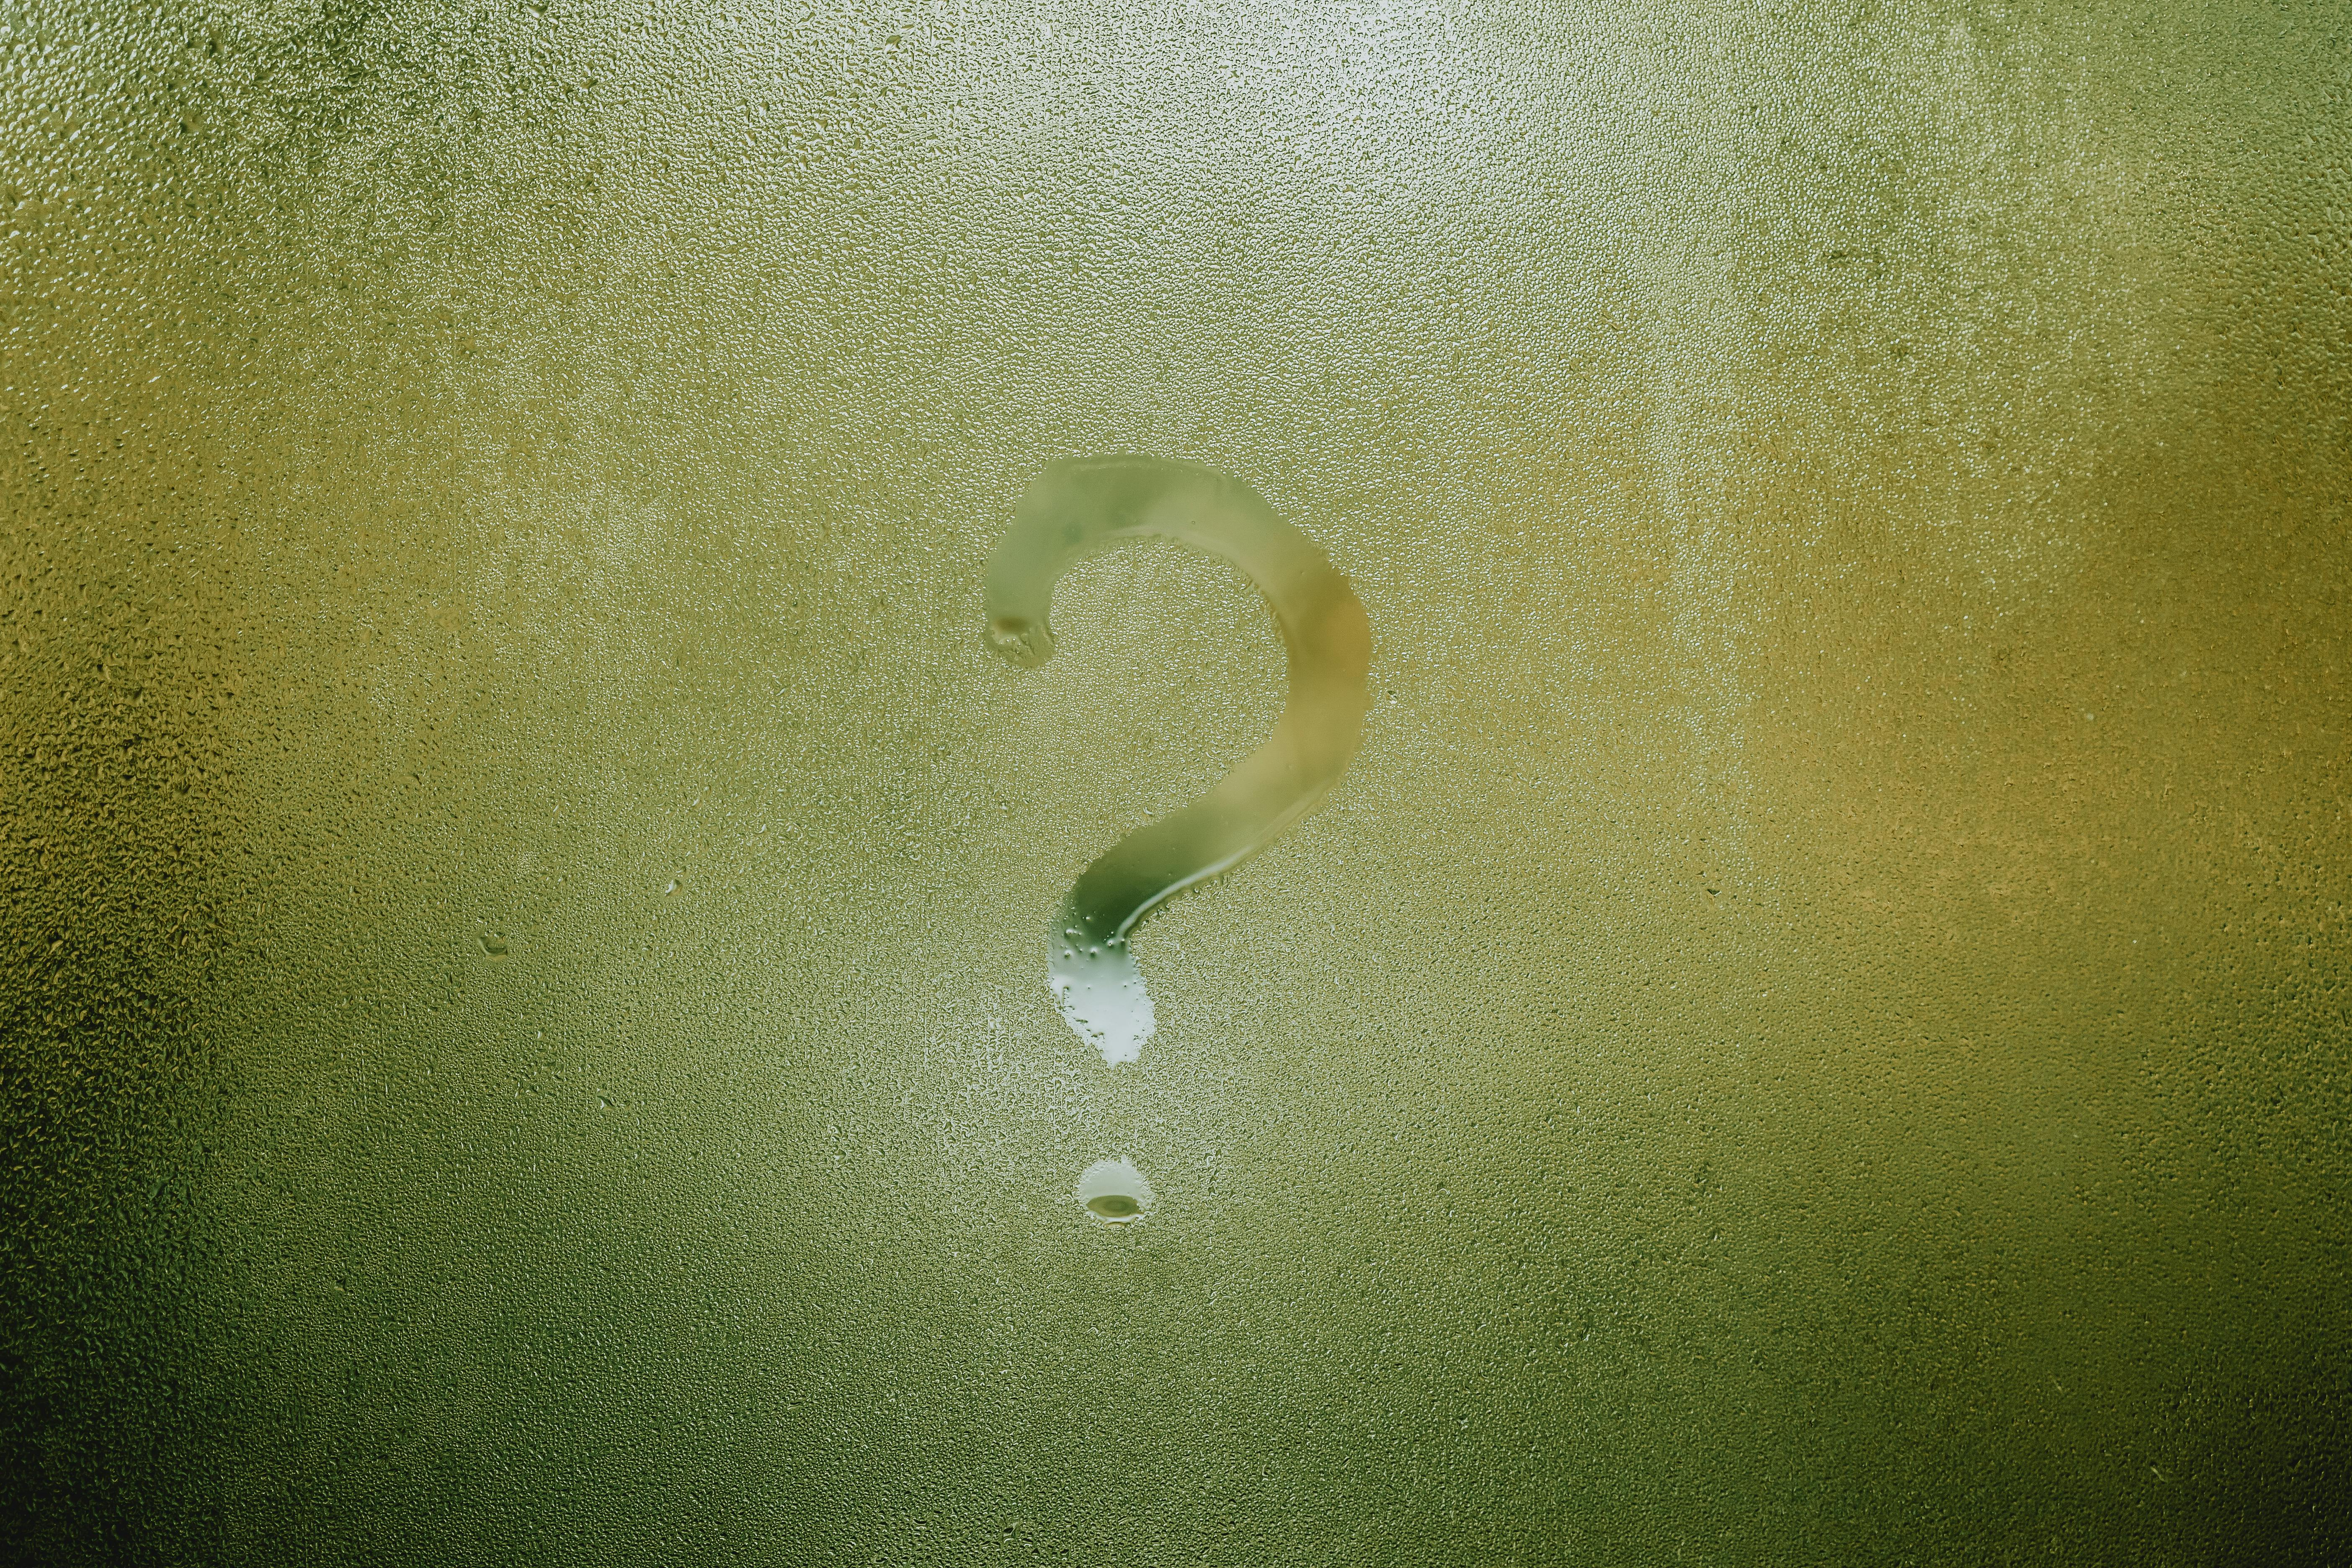
\includegraphics[width=0.6\textwidth]{figs/Interrogacao.jpg}
    \end{figure}
    \vspace{1.7cm}
\end{frame}

% Slide de Agenda
\begin{frame}
    \frametitle{Agenda}
    \tableofcontents
\end{frame}

% Seção 1: Introdução às Redes 5G

\section{Introdução às Redes 5G}
\begin{frame}
    \frametitle{O que é o 5G?}
    \begin{itemize}
        \item Quinta geração de redes móveis.
        \item Promete velocidades ultrarrápidas, latência ultrabaixa e conectividade massiva.
        \item Suporte a novas aplicações, como IoT, realidade aumentada/virtual, veículos autônomos.
    \end{itemize}
\end{frame}

\begin{frame}
    \frametitle{Arquitetura do 5G}
    \begin{itemize}
        \item \textbf{Rede de Acesso por Rádio (RAN)}: Nova radiofrequência e técnicas avançadas de transmissão.
        \item \textbf{Rede Central (Core)}: Baseada em software, mais flexível e ágil.
        \item \textbf{Suporte Multisserviço}: \textit{Network slicing} para diferentes tipos de serviços.
    \end{itemize}
    \begin{figure}
        \centering
        \includegraphics[width=0.7\textwidth]{figs/ArquiteturaGeral5G}
        \caption{Arquitetura Geral do 5G\footcite{5G_architecture}}
    \end{figure}
    \vspace{0.4cm}
\end{frame}

\begin{frame}
    \frametitle{Características Técnicas do 5G}
    \begin{itemize}
        \item \textbf{Velocidade}: Até 20 Gbps.
        \item \textbf{Latência}: Menos de 1 ms.
        \item \textbf{Conectividade Massiva}: Suporte para até 1 milhão de dispositivos por km².
        \item \textbf{Eficiência Espectral}: Utilização otimizada do espectro.
    \end{itemize}
    \begin{figure}
        \centering
        \includegraphics[width=0.5\linewidth]{figs/5G_verticais.png}
        \caption{Requisitos para diferentes tipos de aplicações\footcite{5G_verticais}}
    \end{figure}
\end{frame}


% Seção 2: Tecnologias Habilitadoras do 5G

\section{Tecnologias Habilitadoras do 5G}
\subsection{Redes Definidas por Software (SDN)}

\begin{frame}
    \frametitle{Introdução ao SDN}

    \begin{itemize}
        \item \textbf{Definição}: Arquitetura de rede que separa o plano de controle do plano de dados.
        \item \textbf{Componentes Principais}: Aplicações de rede, controlador SDN, switches programáveis, interfaces.
        \item \textbf{Vantagens}: Flexibilidade, centralização do controle, automação.
    \end{itemize}
    \begin{figure}
        \centering
        \subfloat[Tradicional]{\includegraphics[width=0.45\linewidth]{figs/rede_tradicional.png}}\qquad
        \subfloat[SDN]{\includegraphics[width=0.45\linewidth]{figs/rede_sdn.png}}
        \caption{Redes tradicionais vs SDN\footcite{Plane_Separation}}
        \end{figure}
\end{frame}

\begin{frame}
    \frametitle{Introdução ao SDN}
    \begin{columns}
        \begin{column}{0.55\textwidth}
            \begin{itemize}
                \item \textbf{Plano de Aplicação}: Controle dos recursos via programação.
                \item \textbf{Plano de Controle}: Gerência centralizada dos recursos de rede.
                \item \textbf{Plano de Dados}: Dispositivos de comutação físicos ou virtuais.
                \item \textbf{Interfaces}: Comunicação entre os planos, ao norte (REST), sul (OpenFlow, P4), leste, oeste (API dos controladores).
        \end{itemize}            
        \end{column}
        \begin{column}{0.45\textwidth}
            \vspace{2cm}
            \begin{figure}[h]
                \centering
                \includegraphics[width=0.8\textwidth]{figs/SDN_arquitetura.png}
                \caption{Arquitetura SDN\footcite{Recommended_SDN_Wireless}}
            \end{figure}
        \end{column}
    \end{columns}
\end{frame}

\begin{frame}
    \frametitle{Integração SDN com 5G}
    \begin{itemize}
        \item \textbf{Automação de Redes}: Gerência dinâmica do tráfego e recursos.
        \item \textbf{Casos de Uso}: Redes IoT, redes industriais, redes de campus.
        \item \textbf{Network Slicing}: Criação de fatias para diferentes serviços.
    \end{itemize}
 %    \begin{figure}
 %        \centering
 %        \fbox{
	%    \begin{minipage}{1in}
	% 	  \hfill\vspace{1in}
	%    \end{minipage}
	% }
 %        \caption{Integração SDN e 5G\footcite{Network_Slicing}}	
    % \end{figure}
    \begin{figure}[h]
        \centering
        \includegraphics[width=0.8\textwidth]{figs/Network_Slicing.png}
        \caption{Fatiamento de redes\footcite{Network_Slicing}}
    \end{figure}
\end{frame}

\subsection{Virtualização das Funções de Rede (NFV)}
\begin{frame}
    \frametitle{Introdução ao NFV}
    \begin{itemize}
        \item \textbf{Definição}: Abstração das funções de rede do hardware proprietário, executando-as em servidores padrão.
        \item \textbf{Componentes Principais}: VNF (Funções de Rede Virtualizadas), NFVI (Infraestrutura de Virtualização).
        \item \textbf{Vantagens}: Redução de custos, flexibilidade, rapidez na introdução de serviços.
    \end{itemize}
\end{frame}

\begin{frame}
    \frametitle{Integração NFV com 5G}
    \begin{itemize}
        \item \textbf{Virtualização do EPC (Evolved Packet Core)}: Gestão centralizada e flexível do core da rede.
        \item \textbf{vRAN (Virtualized Radio Access Network)}: Otimização da rede de acesso rádio.
        \item \textbf{Edge Computing}: Suporte a aplicações de baixa latência e alta demanda.
    \end{itemize}
 %    \begin{figure}
 %        \centering
 %        \fbox{
	%    \begin{minipage}{1in}
	% 	  \hfill\vspace{1in}
	%    \end{minipage}
	% }
 %        \caption{Arquitetura NFV no 5G}	
 %    \end{figure}
    % \begin{figure}[h]
    %     \centering
    %     \includegraphics[width=0.8\textwidth]{NFV.png}
    %     \caption{Arquitetura NFV no 5G\footcite{Network_Slicing}}
    % \end{figure}
\end{frame}

% Seção 3: Casos de Uso

\section{Casos de Uso}
\subsection{\textit{Closed-Loop Control} no 5G}
\begin{frame}
    \frametitle{\textit{Closed-Loop Control} (CLC)}
    \begin{itemize}
        \item \textbf{Definição}: Sistema de automação que ajusta parâmetros da rede em tempo real com base em feedback contínuo.
        \item \textbf{Componentes}: Monitoramento, análise, decisão e execução.
        \item \textbf{Benefícios}: Otimização contínua da rede, melhoria na Qualidade de Serviço (QoS), resposta rápida a falhas.
    \end{itemize}
\end{frame}

\begin{frame}
    \frametitle{Aplicações de CLC no 5G}
    \begin{itemize}
        \item \textbf{\textit{Self-Organizing Networks} (SON)}: Redes que se auto-configuram, otimizam e recuperam.
        \item \textbf{Gerenciamento de Tráfego}: Ajustes automáticos para otimizar o fluxo de dados.
        \item \textbf{Manutenção Preditiva}: Prevenção de falhas com base em análise contínua de dados.
    \end{itemize}
\end{frame}

\subsection{Indústria 4.0 e 5G}
\begin{frame}
    \frametitle{Introdução à Indústria 4.0}
    \begin{itemize}
        \item \textbf{Definição}: Fusão de tecnologias digitais, físicas e biológicas, impulsionada pela conectividade e automação.
        \item \textbf{Componentes}: IoT, robótica avançada, \textit{big data}, IA, e computação em nuvem.
        \item \textbf{Objetivo}: Produção mais inteligente, eficiente e flexível.
    \end{itemize}
\end{frame}

\begin{frame}
    \frametitle{O Papel do 5G na Indústria 4.0}
    \begin{itemize}
        \item \textbf{Conectividade Onipresente}: Conexão confiável para um grande número de dispositivos e sensores.
        \item \textbf{Baixa Latência}: Comunicação quase em tempo real, essencial para automação.
        \item \textbf{Customização e Flexibilidade}: Produção adaptável às demandas do mercado.
    \end{itemize}
 %    \begin{figure}
 %        \centering
 %        \fbox{
	%    \begin{minipage}{1in}
	% 	  \hfill\vspace{1in}
	%    \end{minipage}
	% }
 %        \caption{5G e Indústria 4.0}	
 %    \end{figure}
    % \begin{figure}[h]
    %     \centering
    %     \includegraphics[width=0.8\textwidth]{Industry_4.0.png}
    %     \caption{5G e Indústria 4.0}
    % \end{figure}
\end{frame}

\begin{frame}
    \frametitle{Casos de Uso do 5G na Indústria 4.0}
    \begin{itemize}
        \item \textbf{Automação e Robótica}: Robôs conectados em tempo real.
        \item \textbf{Manutenção Preditiva}: Monitoramento contínuo de equipamentos para prever falhas.
        \item \textbf{Supply Chain Inteligente}: Integração e otimização em tempo real de toda a cadeia de suprimentos.
    \end{itemize}
\end{frame}



\input{sections/04_research}

% Seção 5: Hot Topics

\section{Tópicos Quentes de Pesquisa}
\begin{frame}
    \frametitle{Tópicos Quentes de Pesquisa i}
    \begin{itemize}
        \item \textbf{6G e Além}: Exploração de tecnologias para a próxima geração de redes móveis\footcite{6G_beyond}
        \item \textbf{Inteligência Artificial Integrada}: Aplicação de AI/ML para otimização e automação de redes 5G\footcite{AI_5G}
        \item \textbf{Segurança e Privacidade}: Desafios na proteção de dados e na prevenção de ataques cibernéticos em ambientes 5G\footcite{Security_5G}
        \item \textbf{Edge Computing Avançado}: Expansão da capacidade de processamento na borda da rede para suportar aplicações em tempo real\footcite{MEC_5G}
    \end{itemize}
    \vspace{1cm}
\end{frame}

\begin{frame}
    \frametitle{Tópicos Quentes de Pesquisa ii}
    \begin{itemize}
        \item \textbf{Network Slicing Dinâmico}: Desenvolvimento de métodos para alocação e gerenciamento dinâmico de fatias de rede\footcite{Dynamic_NS}
        \item \textbf{Integração com IoT Massivo}: Soluções para lidar com a conectividade de bilhões de dispositivos IoT\footcite{Massive_IoT}
        \item \textbf{Ambientes Virtuais e Realidade Aumentada/Virtual}: Potencial do 5G para suportar experiências imersivas de alta qualidade\footcite{ARVR_5G}
    \end{itemize}
\end{frame}

% Seção 6: Conclusão

\section{Conclusão}
\begin{frame}[allowframebreaks]
    \frametitle{Conclusão}
    \begin{itemize}
        \item A integração SDN/NVF/5G é a base da transformação digital
        \item Flexibilidade e agilidade
        \begin{itemize}
            \item SDN: Controle centralizado e programável da rede.
            \item NFV: Virtualização de funções de rede para rápida implantação e escalabilidade.
        \end{itemize}
        \item Redução de Custos Operacionais
        \begin{itemize}
            \item Menor dependência de hardware proprietário, redução de OPEX e CAPEX.
        \end{itemize}
        \item Automação e Controle em Tempo Real
        \begin{itemize}
            \item SDN: Automação e otimização do tráfego em tempo real.
            \item NFV: Implantação rápida e ajuste de serviços conforme as condições de rede.
        \end{itemize}
        (continua)
        \item Dicas Valiosas
        \begin{itemize}
            \item Aprenda a desenvolver software \\
            {\small
            ``We reject: kings, presidents, and voting. We believe in: rough consensus and running code.'' David Clark, 1992.
            }
            \item Identificar tópicos quentes de pesquisa \\
            {\small CFPs, acompanhar grupos de pesquisa, trabalhos futuros de teses e dissertações etc.}
            \item Publicar é muito importante \\ 
            {\small (\textit{Publish or perish}!!)}
            \item Não brigue com seu orientador \\
            {\small (Apesar de não ser um Jedi, respeite a opnião dele e dos mais experientes)}
            \item A caminhada é muitas vezes mais rica do que o final da trilha
        \end{itemize}
    \end{itemize}
\end{frame}

\begin{frame}[allowframebreaks]
\printbibliography
\end{frame}

\end{document}
